%!TEX root = ../../main.tex

\chapter{Anleitung für Verwaltungsangestellte}
\label{sec:chap2}

\section{Kursübersicht}
Meldet sich ein Dozent bei eCourse an, wird er direkt auf die Kursübersicht geleitet. Auf diese Ansicht kann der Nutzer zu jedem Zeitpunkt zurückkehren, indem er in der Menüleiste den Punkt \glqq Kursübersicht \grqq auswählt. In der Kursübersicht werden dem Nutzer alle Kurse angezeigt, in denen er Mitglied ist. Eine beispielhafte Kursübersicht ist in Abbildung \ref{fib:kursübersicht} gezeigt.

\begin{figure}[h]
\centering
\includegraphics[height=.5\textwidth]{kursübersicht_dozent.png}
\caption{Kursübersicht eines Dozenten in der Anwendung eCourse}
\label{fib:kursübersicht_dozent}
\end{figure}

Möchte der Dozent mehr Informationen zu einem bestimmten Kurs erhalten, erhält er diese, indem er den Kurs in der Kursübersicht ausklappt. Dann werden ihm alle Mitglieder des bestimmten Kurses angezeigt und auch alle Aufgaben, die er dem Kurs gestellt hat. Beispielhaft ist dies in Abbildung \ref{fib:kursübersicht_dozent_ausgeklappt} gezeigt. Genauere Details zu einer Aufgabe erhält der Dozent, indem er in der ausgeklappten Kursübersicht auf die Schaltfläche \glqq anzeigen\grqq\; neben der gewünschten Aufgabe klickt. Genauere Informationen finden sich in Kapitel \ref{sec:herunterladen}. Möchte der Dozent die Aufgabe bearbeiten erreicht er dies indem er auf die Schaltfläche \glqq Bearbeiten\grqq\; klickt. Genauere Informationen dazu finden sich in Kapitel \ref{sec:bearbeiten}
 
\begin{figure}[h]
\centering
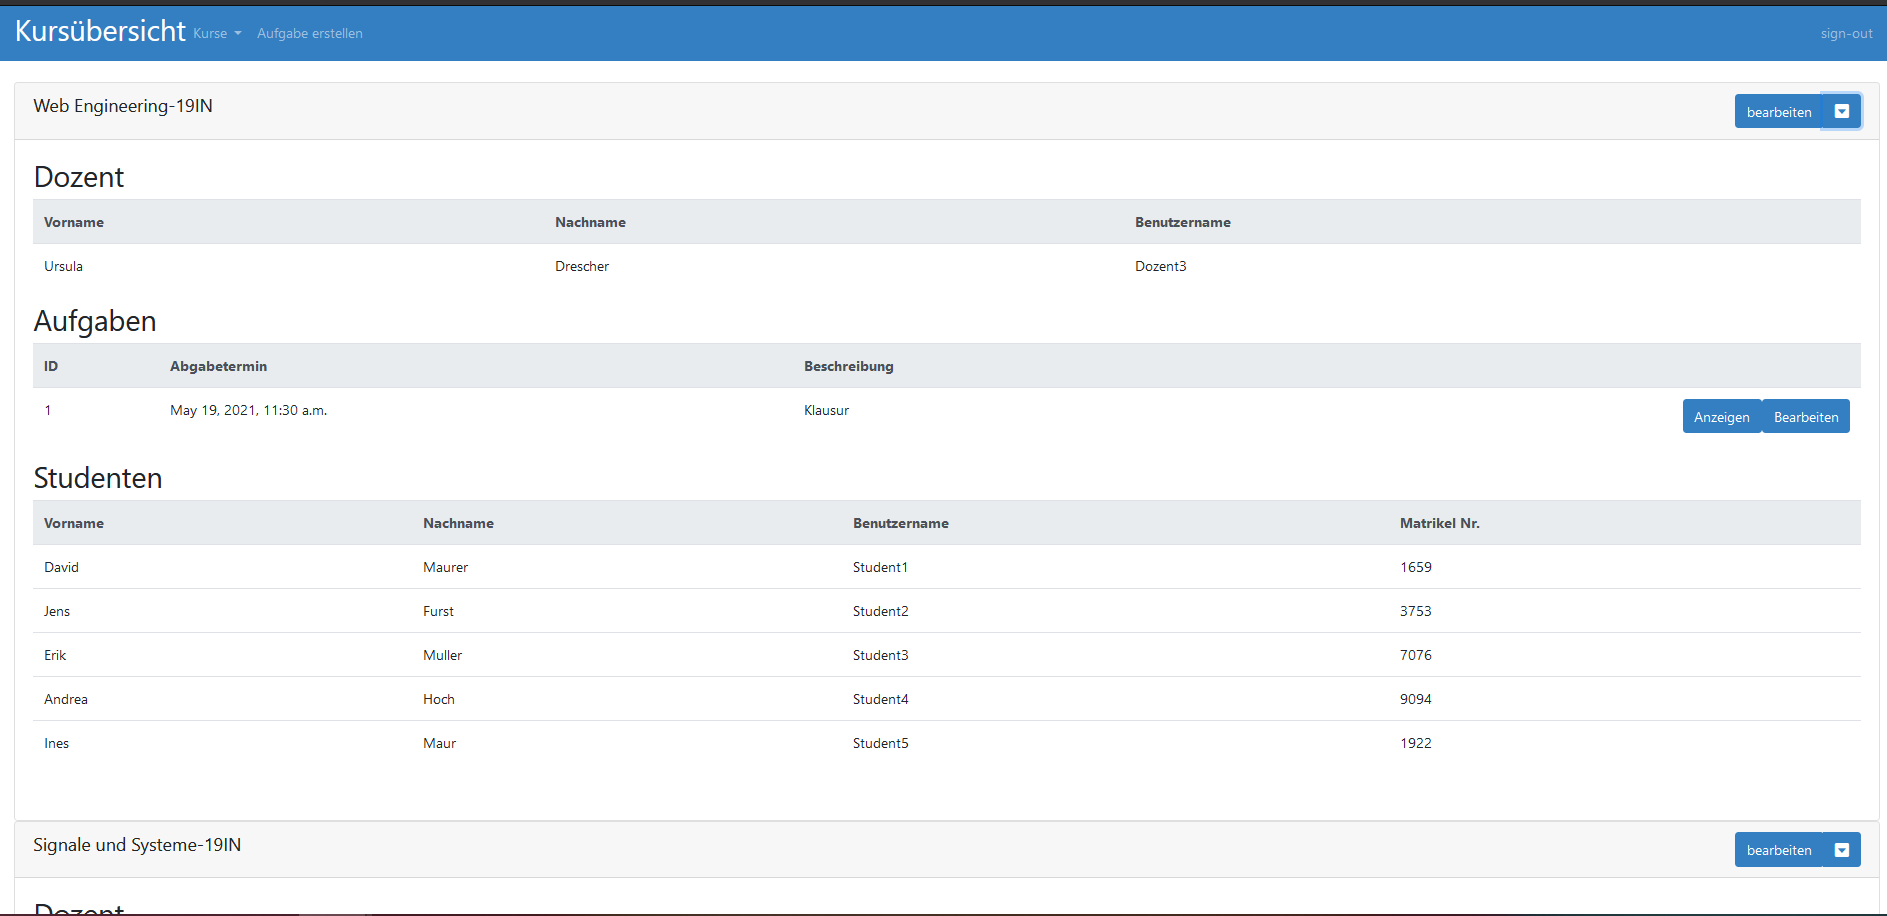
\includegraphics[height=.5\textwidth]{kurse_ausgeklappt_dozent.png}
\caption{Ausgeklappte Kursübersicht eines Dozenten in der Anwendung eCourse}
\label{fib:kursübersicht_dozent_ausgeklappt}
\end{figure}

\section{Kurs erstellen}
Möchte der Dozent selbst einen Kurs erstellen, kann er dies tun, indem er in der Menüleiste den Unterpunkt \glqq Kurs erstellen\grqq\; auswählt. Dadurch gelangt er auf eine Unterseite mit dem entsprechenden Formular um einen Kurs anzulegen. Das Formular ist in Abbildung \ref{fib:kurs_anlegen} gezeigt. Alle Felder des Formulars müssen ausgefüllt sein. Aus der Liste der Dozenten muss der Dozent sich selbst als Dozent des Kurses auswählen.
Die Teilnehmer am Kurs aus der Gruppe der Studierenden werden hinzugefügt, indem man sie anhand ihres Benutzernamens in der Liste ausfindig macht und mit einem Haken versieht. \\
Außerdem sollte dem Kurs sinnvoller Name vergeben werden. Von den Entwicklern wird ein Name empfohlen der dem folgenden Schema entspricht: \\
\verb/Kursname_JJKursbezeichnung/
Abschließend kann über einen Kalender ein Start- und Enddatum des Kurses festgelegt werden. 
Die Erstellung des Kurses kann durch klicken der Schaltfläche \glqq Kurs erstellen\grqq\: beendet werden.

\begin{figure}[h]
\centering
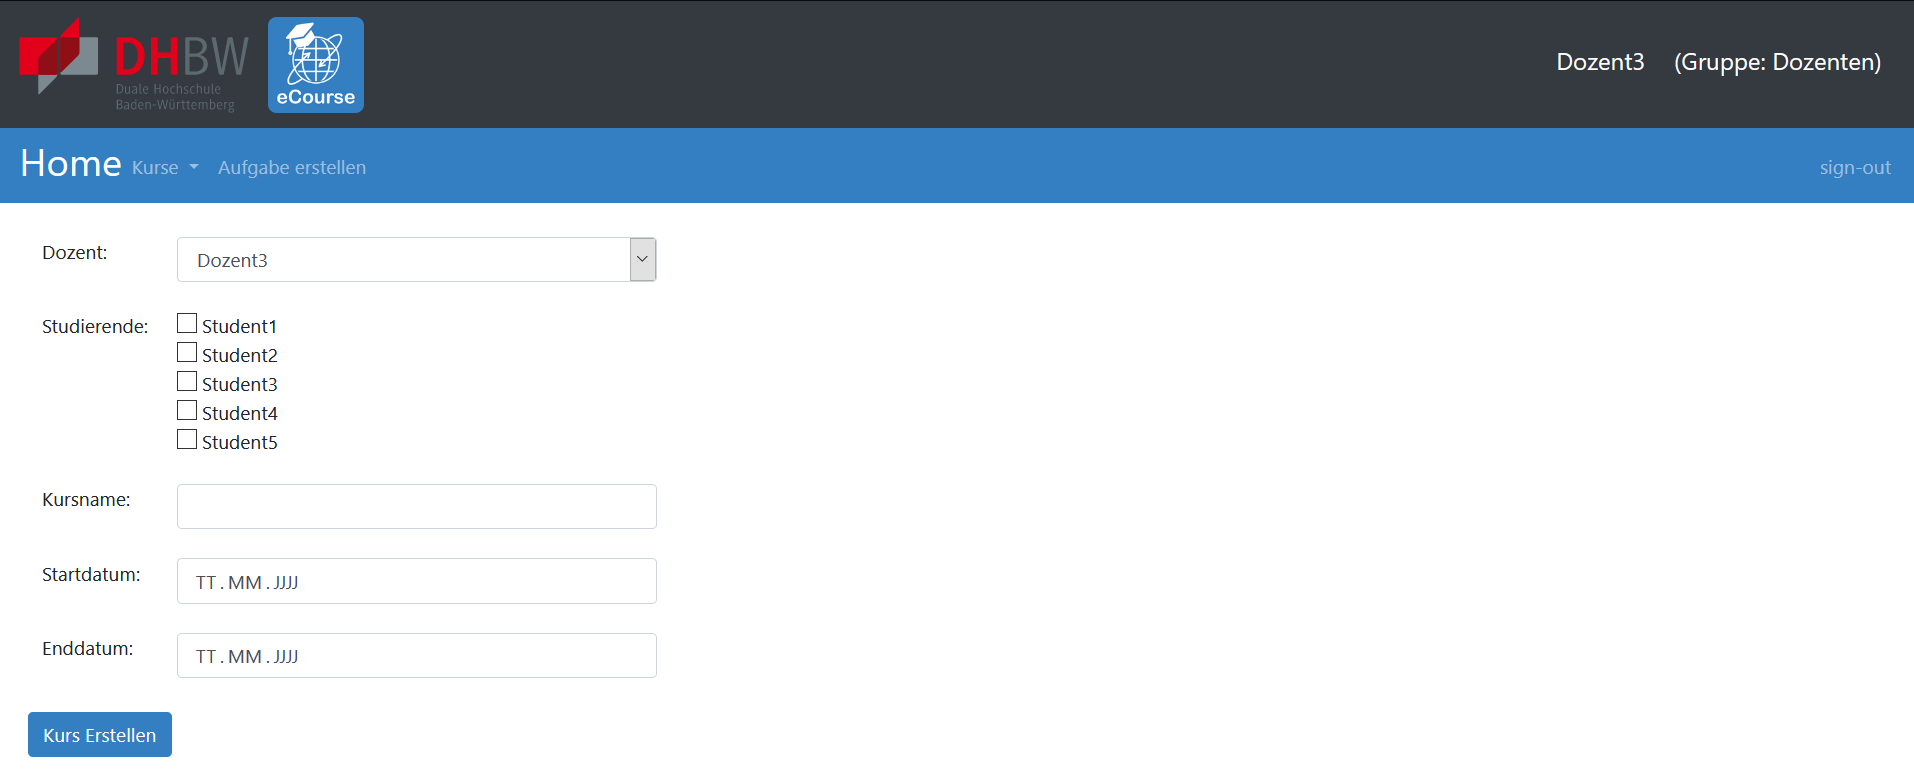
\includegraphics[height=.5\textwidth]{kurs_erstellen_dozent.png}
\caption{Kurs Anlegen durch einen Dozenten in der Anwendung eCourse}
\label{fib:kurs_anlegen}
\end{figure}

\section{Aufgabe erstellen}
Möchte der Dozent den Mitgliedern eines Kurses eine Aufgabe stellen, kann er dies tun, indem er 

\begin{figure}[h]
\centering
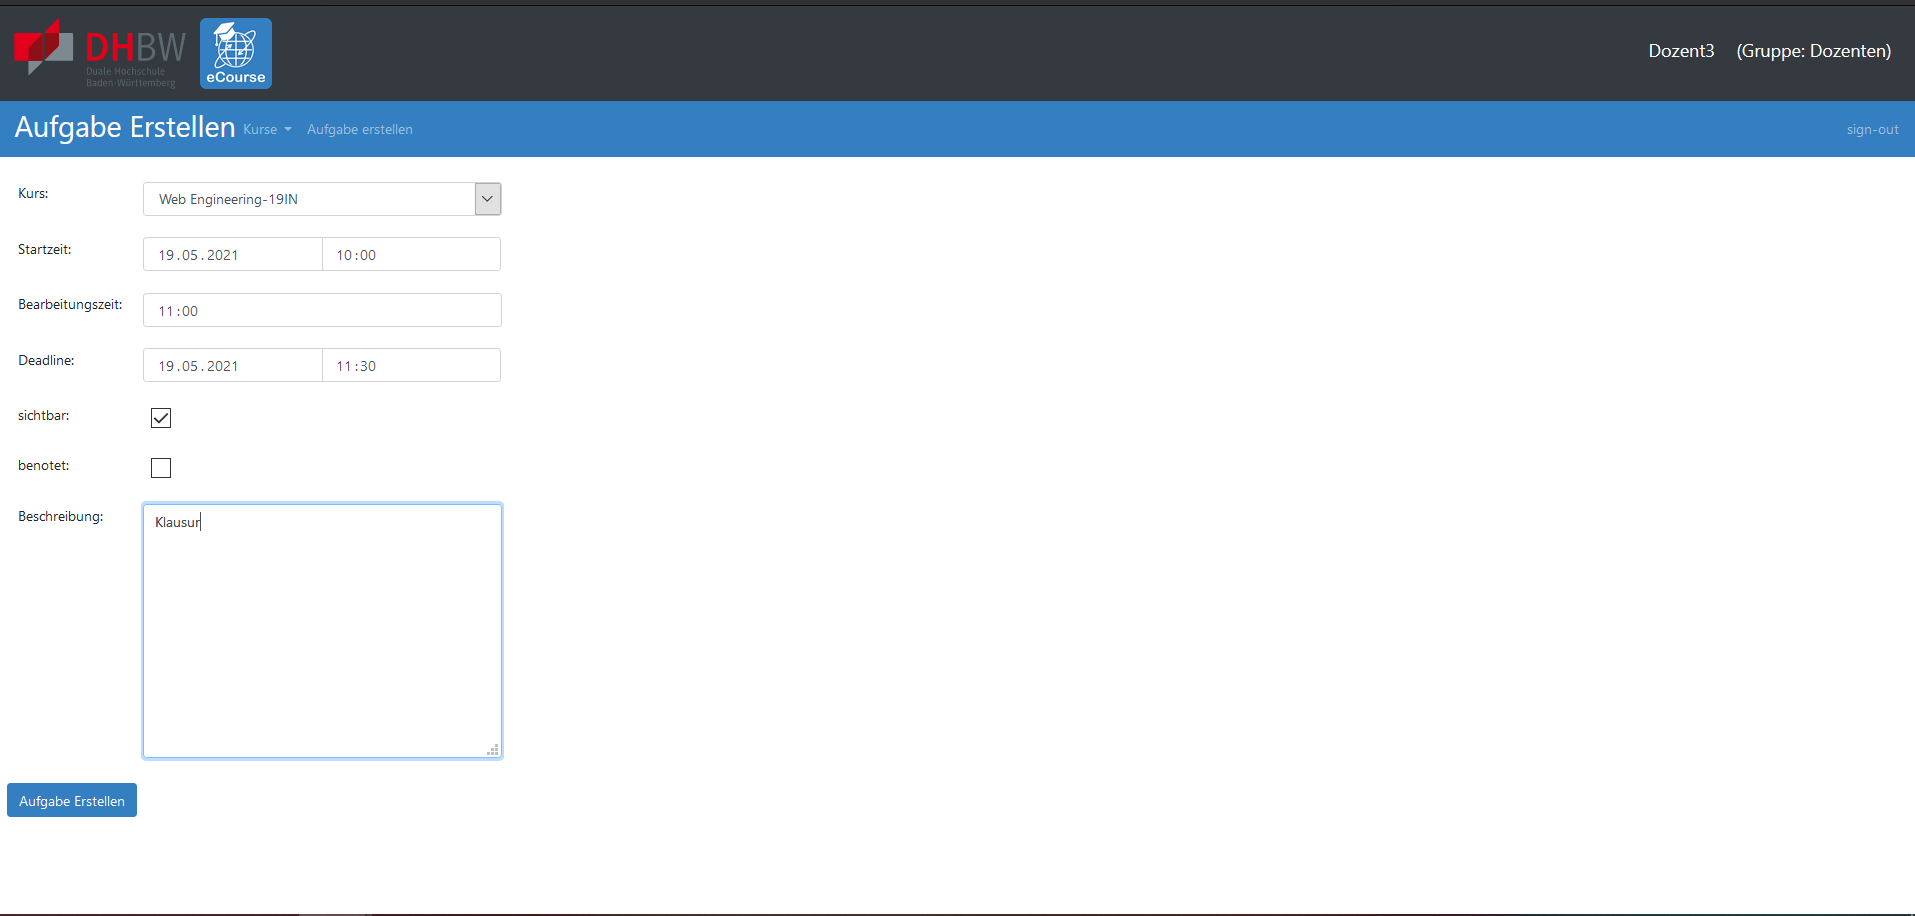
\includegraphics[height=.5\textwidth]{aufgabe_erstellen_dozent.png}
\caption{Aufgabe erstellen in der Anwendung eCourse}
\label{fib:aufgabe_anlegen}
\end{figure}


\section{Aufgabe bearbeiten}
\label{sec:bearbeiten}

\section{Bearbeite Abgaben herunterladen}
\label{sec:herunterladen}